\begin{frame}
  \begin{center}
    \large{Arbres de décision}
  \end{center}
\end{frame}

\begin{frame}
  \frametitle{Exemple}
  \begin{center}
    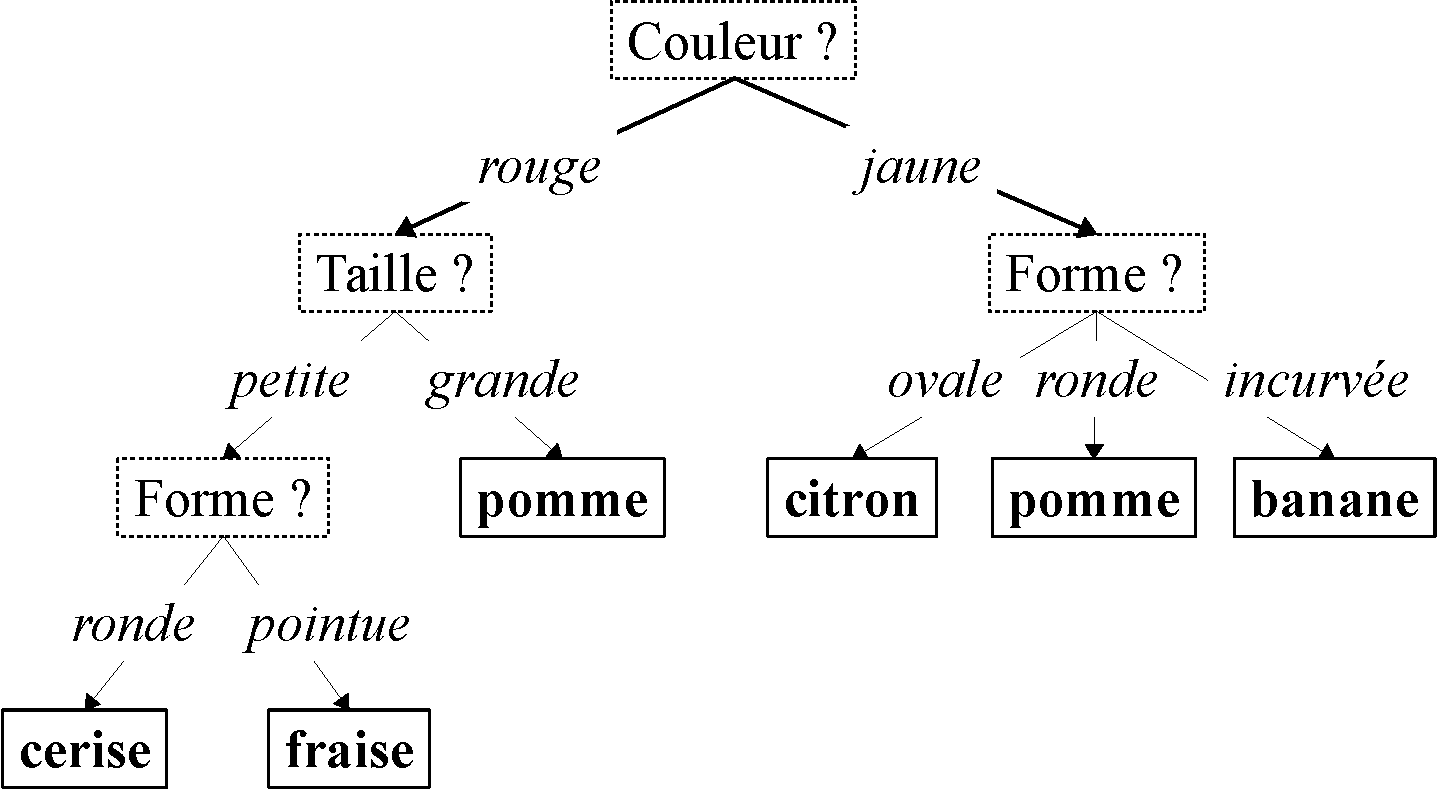
\includegraphics[width=.7\textwidth]{figures/fruit_tree}
  \end{center}
\end{frame}

\begin{frame}
  \frametitle{Les arbres de décision}
  \begin{itemize}
    \item Méthode hiérarchique
    \item Série successive de tests conditionnels.
    \item Souvent utilisé en dehors de la classification automatique : 
    \begin{itemize}
      \item aide à la décision
      \item formalisation d'un raisonnement
    \end{itemize}
  \end{itemize}
\end{frame}


\begin{frame}
  \frametitle{Les arbres de décision pour la classification}
  \begin{center}
    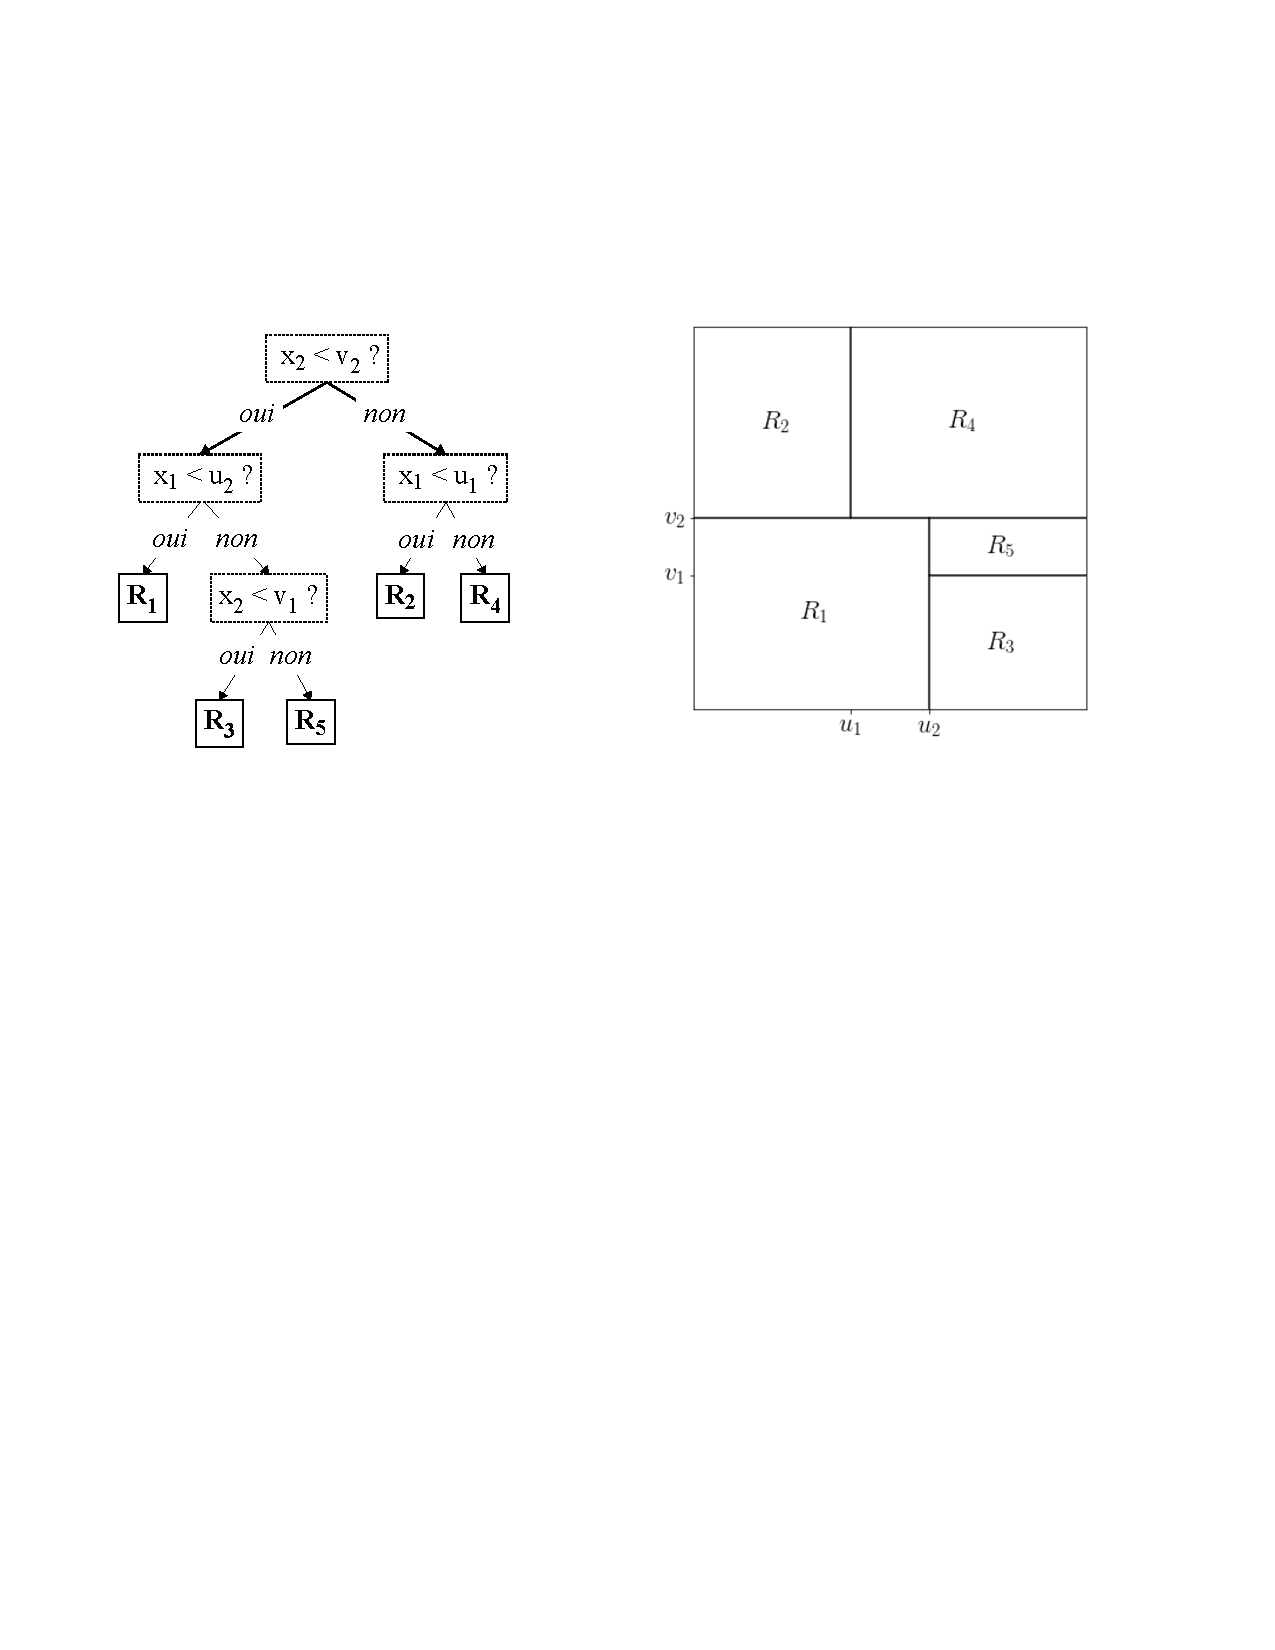
\includegraphics[width=.7\textwidth]{figures/arbre}
  \end{center}
  \begin{itemize}
    \item En classification, les tests correspondent à des seuils, appliqués aux descripteurs. 
    \item Chaque arbre de décision correspond à une partition de l'espace des descripteurs.
    \item On peut assigner une classe à chaque feuille. 
  \end{itemize}
\end{frame}


\begin{frame}
  \frametitle{Les arbres de décision - avantages}
  \begin{itemize}
    \item Classification en classes multiples
    \item Interprétabilité
    \item Traitement de variables catégoriques
    \item Mélange de types de variables
  \end{itemize}
\end{frame}

\begin{frame}
  \frametitle{Construction des arbres}
  \begin{itemize}
    \item CART: Classification and regression trees
    \item A chaque étape, une région est divisée en deux. 
    \item Pour ce, il faut choisir un descripteur $x_j$ et un seuil $s$. 
    \item Ce choix est fait pour optimiser un critère, calculé sur les régions qui résultent de ce seuillage. 
  \end{itemize}
\end{frame}

\begin{frame}
  \frametitle{Split : critère de régression}
  \begin{itemize}
    \item Un suppose qu'un split $(j,s)$ génère deux régions $R_1$ et $R_2$. 
    \item Dans le cas d'une regression, on calcule alors les moyennes $\overline{y_1}$ et $\overline{y_2}$ dans les régions $R_1(j,s)$ et $R_2(j,s)$. 
    \item Le critère à minimiser par $(j,s)$:
    \begin{equation*}
    (j,s)^{\ast} = \argmin_{j,s}\sum_{x_k \in R_1} (y_k-\overline{y_1})^2 + \sum_{x_k \in R_2}(y_k-\overline{y_2})^2
    \end{equation*}
    où $\overline{y_1}, \overline{y_2}, R_1, R_2$ dépendent de $(j,s)$. 
  \end{itemize}
\end{frame}

\begin{frame}
  \frametitle{Split : critère de classification}
  \begin{itemize}
    \item Critère de impureté GINI ; 
    \begin{equation*}
    Imp(R) = \sum_{c=1}^{C}p_c(R)(1-p_c(R))
    \end{equation*}
    avec $p_c(R)$ la probabilité (proportion) de la classe $c$ dans $R$.     
    \item Le critère à minimiser par $(j,s)$:
    \begin{equation*}
    (j,s)^{\ast} = \argmin_{j,s}\frac{|R_1|}{n}Imp(R_1) + \frac{|R_2|}{n}Imp(R_2)
    \end{equation*}
    avec $|\cdot|$ le cardinal et $R_1, R_2$ des fonctions de $(j,s)$. 
  \end{itemize}
\end{frame}

\begin{frame}
  \frametitle{Critère d'arrêt}
  \begin{itemize}
    \item Une classe par feuille : risque de sur-apprentissage
    \item Profondeur fixe
    \item Nombre d'observation par feuille
  \end{itemize}
\end{frame}


% \begin{frame}[t]
%   \frametitle{Construction d'un arbre}
%   \begin{itemize}
%   \item Exemple :
%     \begin{itemize}
%     \item 4 petites pommes jaunes, 5 grosses pommes vertes, 3 bananes, 6 mini-concombres
%     \item attributs : vert/jaune, rond/pas rond, gros/petit
%     \end{itemize}
%   \end{itemize}
% \end{frame}

\begin{frame}
  \frametitle{Limitations}
  \begin{itemize}
    \item Temps de calcul sous-optimal (en inférence)
    \item Grand risque de sur-apprentissage
    \item Généralement une performance limitée
  \end{itemize}
\end{frame}

\begin{frame}
  \begin{center}
    \large{2. Méthodes ensemblistes}
  \end{center}
\end{frame}

\begin{frame}
  \frametitle{Sagesse des foules}
  \begin{center}
    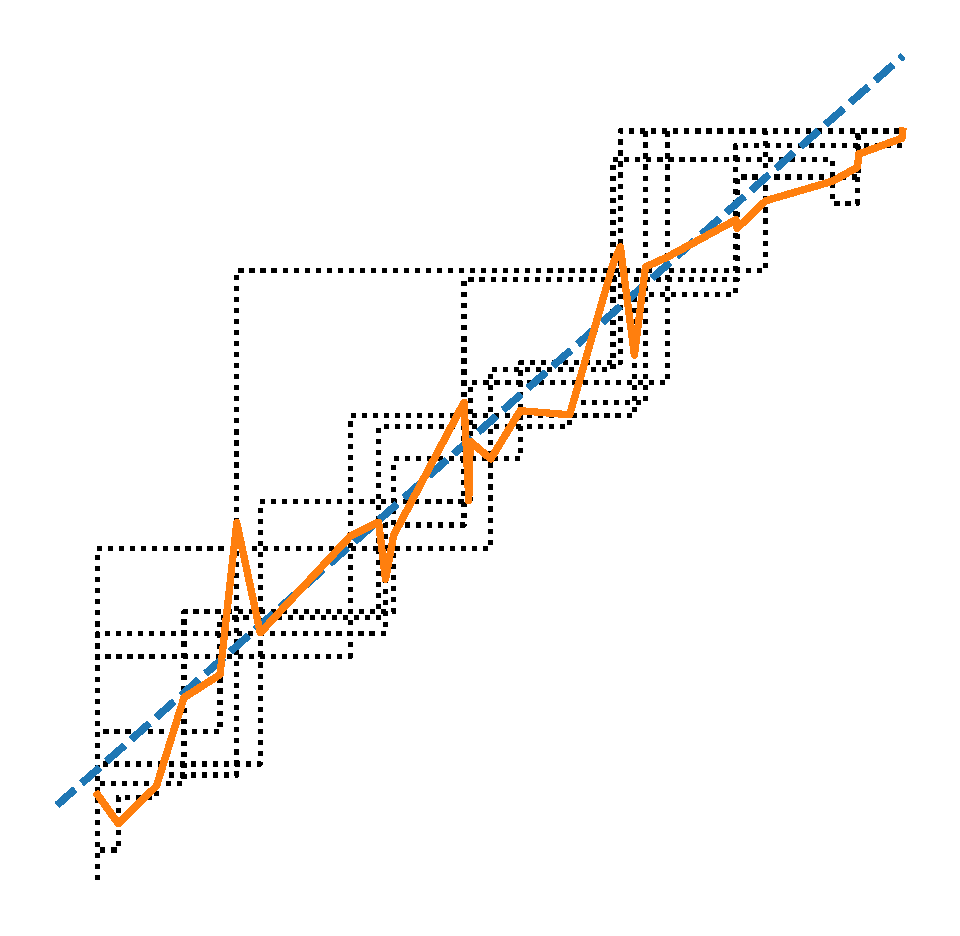
\includegraphics[width=.5\textwidth]{figures/crowd_diagonal}
  \end{center}
  \begin{itemize}
  \item Combiner des \blue{apprenants faibles}.
  \item Exemple: fonction diagonale, approchée par des fonctions en esaclier. 
  \item Principe démocratique. 
  \end{itemize}
\end{frame}

\begin{frame}
  \frametitle{Bagging}
  \begin{itemize}
    \item On considère une partie de $\dset$ (e.g. $80\%$) par échantillonage "bootstrap" (avec remise). 
    \item On entraîne un arbre de décision. 
    \item On reitère cette procédure pour obtenir un ensemble d'arbres. 
    \item Le résultat est obtenu par vote majoritaire (classification) ou en moyennant (régression).  
    \item Faire une moyenne de modèles est effectivement une technique de regression. 
  \end{itemize}
\end{frame}

\begin{frame}
  \frametitle{Forêts aléatoires}
  \begin{itemize}
    \item En plus du bagging, on peut à chaque noeud tirer aléatoirement des variables parmi lesquels la variable optimale est trouvée. 
    \item Le résultat : \blue{les forêts aléatoires}. 
    \item Les arbres sont plus différents et couvrent "différent aspects" des données. 
    \item En pratique : 
    \begin{itemize}
      \item généralement bons résultats sans "tuning"
      \item applicable pour $P \gg N$
      \item Régularisation par "ensembling"
    \end{itemize}
  \end{itemize}

\end{frame}

\begin{frame}
  \frametitle{2.4 Boosting}
  \begin{itemize}
  \item À l'itération $m$
    \begin{itemize}
    \item Apprendre le modèle $f_m$ qui minimise l'erreur empirique de
      \[
        F_m = \sum_{l=1}^m \alpha_l f_l = F_{m-1} + \alpha_m f_m 
      \]
    \item L'erreur pour $(\xvec_i, y_i)$ est pondérée de sorte à donner plus
      d'importances aux exemples pour lesquels $F_{m-1}$ se trompe.
    \end{itemize}
  \item \blue{AdaBoost} (Schapire \& Freund 1997) : erreur exponentielle, $f_m$ est un
    arbre de décision de profondeur 1 (decision stump)
  \item \blue{Gradient Boosting} (Friedman 2001) : forme générale
  \end{itemize}
\end{frame}



%%% Local Variables:
%%% mode: latex
%%% TeX-master: "2022-01-azencott"
%%% End:
